\documentclass[12pt,a4paper]{article}
\usepackage[utf8]{inputenc}
\usepackage[russian]{babel}
\usepackage{amsmath}
\usepackage{amsfonts}
\usepackage{amssymb}
\usepackage{graphics}
\usepackage[pdftex]{graphicx}
\usepackage{lscape}
\author{Анастасия Тарасова}
\title{Отчет по лабораторной работе №1 :\\ \LaTeX{}, Git, GPG}
\begin{document}
\maketitle
\section{Система верстки \TeX{} и расширения \LaTeX{}}
\subsection{Цель работы}
Освоить систему верстки \TeX{} и сделать отчет.
\subsection{Ход работы}
В ходе работы был создан файл с расширением .tex, в котором содержатся команды текстовой разметки.
\subsubsection{Компиляция в командной строке}
\subsubsection{Оболочка TexMaker}
TexMaker - текстовый редактор, работающий с языком разметки LaTeX. TexMaker позволяет работать с фишками профессионального оформления. Внешний вид редактора представлен на рисунке 1.
\begin{figure}[h!]
\centering
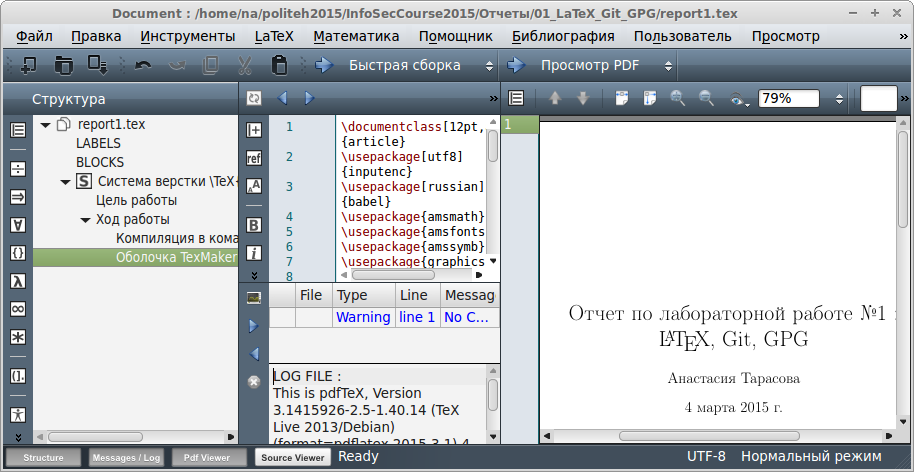
\includegraphics[scale=0.4]{res/texmaker}
\caption{Редактор TexMaker}
\end{figure}
\end{document}
